\documentclass[10pt,a4paper]{article}
\usepackage[utf8]{inputenc}
\usepackage{amsmath}
\usepackage{amsfonts}
\usepackage{amssymb}
\usepackage{graphicx}
\usepackage{fancyhdr}
\usepackage{siunitx}
\pagestyle{fancy}
\fancyhead{}
\fancyhead[L]{\slshape MCTS Mario}
\fancyhead[R]{\slshape IT University of Copenhagen}
\fancyfoot{}
\fancyfoot[C]{\thepage}
%\graphicspath{ {C:\Users\Rasmus\workspace\MCTSMario\Rapport} }
\renewcommand{\si}[1]{\SI{#1}}

\begin{document}
\title{Enhancements for Monte Carlo Tree Search in The Mario AI Framework}
\date{May 22, 2013}
\author{Emil Juul Jacobsen\\\texttt{ejuu@itu.dk}        
        \and Rasmus Greve\\\texttt{ragr@itu.dk}}
%TODO    \and \emph{Supervisor:}\\Julian Togelius\\\texttt{juto@itu.dk}}
\maketitle
\thispagestyle{empty} %Removes default pagenumber from frontpage

\begin{abstract}
(Bare copy/paste-ish fra projektbasen, skal skrives om!) %TODO
In this experiment we explore different implementations and enhancements of the Monte Carlo Tree Search algorithm for an AI, in order to evaluate their performance and results in the Super Mario AI Benchmark tool. 
We have implemented the basic MCTS algorithm in the Mario AI 
Framework and characterised the performance and identification of 
the strengths and weaknesses of the algorithm relative to the 
framework. We have identified a set of refinements and alterations of the algorithm 
and through implementation and evaluation of these individually we came up
with compositions that greatly increase the performance of the AI.
\end{abstract}
\clearpage

\section{Introduction}
In this experiment we explore different implementations and enhancements of the Monte Carlo Tree Search (MCTS) algorithm for an AI, in order to evaluate their performance and results in the Super Mario AI Benchmark tool \cite{mario}. The MCTS algorithm has shown great results in various classical board games but has (to our knowledge) not been tested on a real-time physics-based game like Super Mario. Like some of the games that MCTS has proven effective in, Super Mario has a large branching factor of the state space but differs in that simulating actions is quite computationally expensive. These differences make several modifications of the core algorithm interesting for our experiment because they can help build the tree in a manner that uses the simulations more effectively. %TODO
\clearpage

\section{Background}
%TODO Fill this space
\subsection{Monte Carlo Tree Search}

Monte Carlo Tree Search has shown surprisingly good results in solving problems with large branching factors. MCTS is a tree search algorithm, where evaluation of a node is done by random sampling in the decision space until an outcome can be determined. A very nice property of MCTS is that it is an \emph{anytime} algorithm, meaning that it can be halted when a time budget is reached and give the result that looks the most promising at the given time. Furthermore it often requires no or very little domain knowledge as a basic implementation only require knowledge of the action space and a means of simulating the outcome of an action.


Searching in MCTS is done by iteratively by building a search tree where the nodes are game states, and the edges are actions. A node is added to the tree in each iteration and recursively, based on the reward of the new node, the reward of parent nodes are updated.
A single iteration of the MCTS building process consists of these four steps:
\begin{enumerate}
\item Tree Policy (A node to be expanded is chosen)
\item Expansion (The node is expanded by simulating the associated action)
\item Default Policy (The game is simulated with random moves until terminal)
\item Backpropagation (The result propagates up through the tree)
\end{enumerate}
Modifications to this core algorithm will change one or more of these steps. We will note for each modification what steps they modify.
\subsubsection{Tree Policy}
In the beginning of each iteration the algorithm must search through the tree and determine which existing node to expand. This is done by traversing the tree until we find a node that is not fully expanded. Modifications to this part of the algorithm generally differs in the choice between existing child nodes when looking at a fully expanded node.
\subsubsection{Expansion}
From the node that is not fully expanded a new child node is created corresponding to performing a specific action to the state of the current node. Differences in policies here are due to selecting the new child and how the action is performed (e.g. section \ref{macro}).
\subsubsection{Default Policy}
The default policy determines what is done leading up to the final calculation of the reward for the new node. For the basic MCTS this consist of doing random actions until we reach a terminal state which could either be a win or a loss.
\subsubsection{Backpropagation}
The final reward calculated after performing the default policy is saved in the node, and propagated up the tree to all ancestors. This value will then be used by the tree policy in later iterations. Changes to backpropagation differ in the way that the value of the parent node is altered by the newly calculated value of the child

\subsection{Upper Confidence Bounds for Trees}
Choosing which node to expand can be done in multiple ways. Upper Confidence Bound (UCB) is a bandit based approach to choosing the most urgent node to expand. The quality with UCB is that it allows for prioritizing between exploration of less tried nodes, and exploitation of seemingly promising nodes.
\begin{equation}
\label{eq:ucb1}
\displaystyle UCB_j = \overline{X}_j + \sqrt{\frac{2 * \log(n)}{n_j}}
\end{equation}
Here $X_j$ is the average (i.e. expected) reward. $n$ is the total number of plays and $n_j$ is the number of times action $j$ was tried. Since the exploration term of the equation depends on how explored the node is compared to the parent, the confidence in a node will increase steadily until the node is eventually explored. The exploitation term will, however, make sure that good nodes will be explored more frequently than less promising ones.

\subsection{The Mario AI Framework}
The framework we use to test our different artificial intelligences is called The Mario AI Benchmark 2009\cite{mario}. Through this framework we are able to implement the various AI algorithms in Java, test their performance and finally compare it to existing AIs.
\subsubsection{The Game API}
The interface required to implement an Agent is actually quite simple containing only five method where only 2 is relevant for the actual AI.

The first method is simply \emph{reset()} that when called instructs the agent to reset all their internal content and prepare for a new simulation. This method is important for the benchmarking of the agents where the agent is playing several games consecutively.

The single most important method is, however, \emph{getAction(Environment obs)}. This is where the agent actually does the calculations necessary to take an intelligent decision. In order for the game to run in real-time the agent can not use more than \si{40}{ms} since that would push the game below 25 frames per second.

The \emph{Environment} provided to the agent contains all the information currently visible on the screen. The primary content of this environment is a matrix of the area surrounding Mario, Mario's coordinates and an array of coordinates for all enemies currently on the screen. The to-dimensional matrix of the environment has a width and height of 22 with Mario centered at the coordinates 11,11. Each cell contains the number for what type of terrain is at that location, these could mean ground, box, cannon-tower etc.

The global coordinates provided for Mario can, with the enemy coordinates, be useful for determining how close he is to danger, and in our case to set up a correct simulation.

With this information the agent is required to give an action back, which is the combination of buttons that Mario will press at this point of time. There are five different buttons available in this game; Left, Right, Down, Jump and Speed. The choices for these buttons are returned from the agent as an array with a boolean for each button.
\subsubsection{Performance measurement}
\label{benchmark}
Apart from simply running and visualizing the game, the framework also includes a benchmarking tool called \emph{Stats}. When running this program with a given agent it will run 800 games of Super Mario at varying difficulty and from the results of these playthroughs it will calculate a final score for the agent. This score is based on the minimum, maximum and average score on the different difficulty levels, and is thereby actually independent of the number of games played at each difficulty. We have created a modification of this tool (\emph{MiniStats}) where each difficulty level is played fewer times, reducing the time needed for a benchmarking from 6 hours to about 30 minutes. The results from these test are valuable for getting an idea about the performance of a modification, but definitely gives a less conclusive result.

Using this tool on different implementations of the agent will provide a fair comparison between them, enabling us to evaluate our different implementations against each other, and finished external agents.

\subsection{Foundation}
The MCTS algorithm requires a correct simulation of future actions in order to determine what action lead to the best outcome. Therefore we are using the simulation classes by Robin Baumgarten extracted from the benchmark tool itself. This simulations lets us keep a game state for each tree node of our simulation and when needed we can copy the state, set the next action for Mario and progress the simulation one tick further.

We also noticed that Baumgarten had problems with the gaps in his A* solution, and because of that the simulation includes information of whether or not Mario is currently inside a gap. We have chosen to use this small piece of code instead of calculating it again ourselves (In section \ref{hole}).

\clearpage

\section{Approach and Enhancements}
In this section we will go over the different implementations and enhancements that we have experimented with. For enhancements including a value that can be tweaked we have tried finding the optimal setting, and in the end we have combined enhancements which complement each other well.

\subsection{Monte Carlo Tree Search with UCB}
To have a baseline for comparison and an implementation to build on, we started by implementing the basic Monte Carlo Tree Search algorithm with Upper Confidence Bounds for selection of nodes. It is evident that many basic implementations of MCTS includes UCT\cite{mspacman}, which also makes good sense in our context, due to the positive effect of a tree unbalanced towards the best nodes.

\subsubsection{Description}
The characteristics of basic MCTS with UCB are that 

Source \cite{mctssurvey}

\subsubsection{Implementation}

\subsubsection{Behaviour}

\subsection{Domain knowledge}
While MCTS on it's own does show some intelligent behaviour, we felt like we had to introduce some domain knowledge to the algorithm to make it perform better. Otherwise most of the enhancements to make wouldn't really show much difference, as it in any case would lead to quite a large amount of random behaviour.

\subsubsection{Description}
\paragraph{Down button}
The absolute first piece of domain knowledge that we introduced was to remove the possibility of pressing the down arrow making Mario duck. In a very few cases it indeed does make sense to duck - under a bullet or a flying monster - but while it can be of use, it also doubles the action space from 16 to 32 possible actions which reduces the reachable depth significantly.
Another important factor that made us disable the down button was that while the down button is pressed, pressing left or right does not make Mario move.

\paragraph{Specific actions}
Blablabla om specifikke actions

\paragraph{Hole Detection}
\label{hole}
Blablabla om hole detection

\subsubsection{Implementation}

\paragraph{Down button and specific actions}
Blablabla om specifikke actions
\paragraph{Hole detection}
Blablabla om hole detection

\subsubsection{Behaviour}

\paragraph{Down button and specific actions}
Blablabla om specifikke actions
\paragraph{Hole detection}
Blablabla om hole detection

%---------------------------------------------------------
\subsection{Softmax Backup}
\subsubsection{Description}
\begin{equation}\label{eq:softmax_equation}
exploitation = Q * maxReward + (1 - Q ) * averageReward
\end{equation}
We use equation \ref{eq:softmax_equation} to calculate the exploration part for the confidence of nodes

\subsubsection{Implementation}

\subsubsection{Behaviour}

%---------------------------------------------------------
\subsection{Macro actions}
\label{macro}
\cite{salesman}
\subsubsection{Description}
\subsubsection{Implementation}
\subsubsection{Behaviour}
%---------------------------------------------------------
\subsection{Heuristic Partial Tree Expansion Policy}
\subsubsection{Description}
\subsubsection{Implementation}
\subsubsection{Behaviour}
%---------------------------------------------------------
\subsection{Checkpoints}
\subsubsection{Description}
\subsubsection{Implementation}
\subsubsection{Behaviour}
%---------------------------------------------------------
\subsection{(Combination)}
\subsubsection{Description}
\subsubsection{Implementation}
\subsubsection{Behaviour}

\clearpage

\section{Results}
\renewcommand{\arraystretch}{1.5}
\begin{table}[h]
	\centering
	\begin{tabular}{| l | l |}
		\hline
		\textbf{Method} & \textbf{Score} 		\\ \hline
		Softmax backup q = 0 (UCT) 			& - \\ \hline
		Softmax backup q = $\frac{1}{8}$	& - \\ \hline
		Softmax backup q = $\frac{1}{4}$	& - \\ \hline
		Softmax backup q = $\frac{1}{2}$	& - \\ \hline
		Softmax backup q = 1 (Max)			& - \\ \hline
	\end{tabular}
	\caption{Results of using Softmax backup with different q values}
	\label{tab:softmax_results}
\end{table}

\begin{table}[h]
	\centering
	\begin{tabular}{| l | l | l |}
		\hline
		\textbf{Method} & \textbf{Avg. number of nodes} & \textbf{Score} \\ \hline
		MCTS w/ UCT, limit = 0			& - & - \\ \hline
		MCTS w/ UCT, limit = 1			& - & - \\ \hline
		MCTS w/ UCT, limit = 2			& - & - \\ \hline
		MCTS w/ UCT, limit = 4			& - & - \\ \hline
		MCTS w/ UCT, limit = 8			& - & - \\ \hline
		MCTS w/ UCT, limit = 16			& - & - \\ \hline
		MCTS w/ UCT, limit = $\infty$	& - & - \\ \hline
	\end{tabular}
	\caption{Results of using UCT with a different limit for random moves}
	\label{tab:uct_results}
\end{table}

\begin{table}[h]
	\centering
	\begin{tabular}{| l | l |}
		\hline
		\textbf{Method} & \textbf{Score} \\ \hline
		MCTS w/ UCT, cp = 0			 			& - \\ \hline
		MCTS w/ UCT, cp = $\frac{1.5}{8}$		& - \\ \hline
		MCTS w/ UCT, cp = $\frac{1}{4}$		 	& - \\ \hline
		MCTS w/ UCT, cp = $\frac{1}{3}$		 	& - \\ \hline
		MCTS w/ UCT, cp = $\frac{1}{2}$		 	& - \\ \hline
		MCTS w/ UCT, cp = $\frac{1}{\sqrt{2}}$	& - \\ \hline
		MCTS w/ UCT, cp = $2$			 		& - \\ \hline
		MCTS w/ UCT, cp = $5$			 		& - \\ \hline
		MCTS w/ UCT, cp = $10$		 			& - \\ \hline
	\end{tabular}
	\caption{Results of using UCT with different weight between exploration and exploitation}
	\label{tab:uct_cp_results}
\end{table}

\begin{table}[h]
	\centering
	\begin{tabular}{| l | l |}
		\hline
		\textbf{Method} & \textbf{Score} \\ \hline
		UCT (Softmax q = 0)				& - \\ \hline
		Max (Softmax q = 1)				& - \\ \hline
		Softmax							& - \\ \hline
		Limited Actions		 			& - \\ \hline
		Hole Detection		 			& - \\ \hline
		Macro Actions		 			& - \\ \hline
		H. Partial Expansion			& - \\ \hline
		Checkpoints						& - \\ \hline
		(Combination)					& - \\ \hline
	\end{tabular}
	\caption{Results from all the different enhancements}
	\label{tab:method_results}
\end{table}


\begin{figure}[h]
\centering
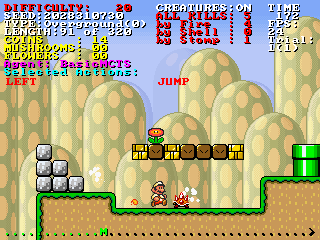
\includegraphics[width=6cm]{Forfulgt.png}
\caption{Mario being followed}
\label{fig:followed}
\end{figure}

Her er noget mere tekst, reference til figur \ref{fig:followed}
\clearpage
\section{Conclusion}
\clearpage

\begin{thebibliography}{9}
\bibitem{mctssurvey}
  C. B. Browne, E. Powley, D. Whitehouse, S. M. Lucas, P. I. Cowling, P. Rohlfshagen, S. Tavener, D. Perez, S. Samothrakis, and S. Colton, “A survey of monte carlo tree search methods,” Computational Intelligence and AI in Games, IEEE Transactions on, vol. 4, no. 1, pp. 1–43, 2012.

\bibitem{civii}
S. R. K. Branavan, D. Silver, and R. Barzilay, “Non-linear monte-carlo search in civilization ii,” in Proceedings of the Twenty-Second international joint conference on Artificial Intelligence-Volume Volume Three, 2011, pp. 2404–2410.

\bibitem{salesman}
E. J. Powley, D. Whitehouse, and P. I. Cowling, “Monte Carlo Tree Search with macro-actions and heuristic route planning for the Physical Travelling Salesman Problem,” in Computational Intelligence and Games (CIG), 2012 IEEE Conference on, 2012, pp. 234–241.

\bibitem{mspacman}
T. Pepels and M. H. Winands, “Enhancements for Monte-Carlo Tree Search in Ms Pac-Man,” in Computational Intelligence and Games (CIG), 2012 IEEE Conference on, 2012, pp. 265–272.

\bibitem{mario}
S. Karakovskiy and J. Togelius, “The mario ai benchmark and competitions,” Computational Intelligence and AI in Games, IEEE Transactions on, vol. 4, no. 1, pp. 55–67, 2012.

\end{thebibliography}

\end{document}